\documentclass[review=true, 10pt, sigplan]{acmart}
\usepackage[utf8]{inputenc}
\usepackage[T1]{fontenc}

\newcommand{\packageGraphicx}{\usepackage{graphicx}}
\newcommand{\packageHyperref}{\usepackage{hyperref}}
\newcommand{\renewrmdefault}{\renewcommand{\rmdefault}{ptm}}
\newcommand{\packageRelsize}{\usepackage{relsize}}
% amsmath is required for the combination of {mathabx,
% wasysym, newtxmath} to work. Otherwise, newtxmath
% would load amsmath *after* mathabx and wasysym,
% causing command redefinition issues.
\newcommand{\packageAmsmath}{\usepackage{amsmath}}
\newcommand{\packageMathabx}{\usepackage{mathabx}}
% Avoid conflicts between "mathabx" and "wasysym",
% and between "wasysym" integrals and "amsmath" integrals (iint).
\newcommand{\packageWasysym}{
  \let\leftmoon\relax \let\rightmoon\relax \let\fullmoon\relax \let\newmoon\relax \let\diameter\relax
  \usepackage[nointegrals]{wasysym}}
% Both newtxmath and mathabx define the \widering command.
% The only reason we choose the newtxmath version is that
% acmart.cls is also using the one from newtxmath.
\newcommand{\packageTxfonts}{
  \let\widering\relax
  \let\oldwidebar\widebar
  \let\widebar\relax
  \usepackage{newtxmath}
  % if newtxmath is before version 1.7.0,
  % then we are still going to use widebar from mathabx
  \ifx\widebar\relax
    \let\widebar\oldwidebar
  \fi
}
\newcommand{\packageTextcomp}{\usepackage{textcomp}}
\newcommand{\packageFramed}{\usepackage{framed}}
\newcommand{\packageHyphenat}{\usepackage[htt]{hyphenat}}
\newcommand{\packageColor}{\usepackage[usenames,dvipsnames]{color}}
\newcommand{\doHypersetup}{\hypersetup{bookmarks=true,bookmarksopen=true,bookmarksnumbered=true}}
\newcommand{\packageTocstyle}{}
\newcommand{\packageCJK}{\IfFileExists{CJK.sty}{\usepackage{CJK}}{}}
%%%%%%%%%%%%%%%%%%%%%%%%%%%%%%%%%%%%%%%%%%%%%%%%%%%%%%%%%%%%%%%%%%%%%%%%%%%%%%%%
% BEGIN acmart-load.tex
% Avoid package option conflict
\renewcommand\packageColor\relax
\renewcommand\packageTocstyle\relax
\renewcommand\packageMathabx{\ifx\bigtimes\undefined \usepackage{mathabx} \else \relax \fi}
% Both 'mathabx' and 'newtxmath' (required by the 'acmart' class) define a '\bigtimes' command. 
\renewcommand\packageTxfonts\relax
\let\Footnote\undefined
\let\captionwidth\undefined
\renewcommand{\renewrmdefault}{}
% END acmart-load.tex
%%%%%%%%%%%%%%%%%%%%%%%%%%%%%%%%%%%%%%%%%%%%%%%%%%%%%%%%%%%%%%%%%%%%%%%%%%%%%%%%
% This is the default style configuration for Scribble-generated Latex

\packageGraphicx
\packageHyperref
\renewrmdefault
\packageRelsize
\packageAmsmath
\packageMathabx
\packageWasysym
\packageTxfonts
\packageTextcomp
\packageFramed
\packageHyphenat
\packageColor
\doHypersetup
\packageTocstyle
\packageCJK


%%%%%%%%%%%%%%%%%%%%%%%%%%%%%%%%%%%%%%%%%%%%%%%%%%%%%%%%%%%%%%%%%%%%%%%%%%%%%%%%
% Configuration that is especially meant to be overridden:

% Inserted before every ``chapter'', useful for starting each one on a new page:
\newcommand{\sectionNewpage}{}
% Inserted before every book ``part''
\newcommand{\partNewpage}{\sectionNewpage}

% Hooks for actions within the `document' environment:
\newcommand{\preDoc}{}
\newcommand{\postDoc}{}

% Generated by `secref'; first arg is section number, second is section title:
\newcommand{\BookRef}[2]{\emph{#2}}
\newcommand{\ChapRef}[2]{\SecRef{#1}{#2}}
\newcommand{\SecRef}[2]{section~#1}
\newcommand{\PartRef}[2]{part~#1}
% Generated by `Secref':
\newcommand{\BookRefUC}[2]{\BookRef{#1}{#2}}
\newcommand{\ChapRefUC}[2]{\SecRefUC{#1}{#2}}
\newcommand{\SecRefUC}[2]{Section~#1}
\newcommand{\PartRefUC}[2]{Part~#1}

% Variants of the above with a label for an internal reference:
\newcommand{\BookRefLocal}[3]{\hyperref[#1]{\BookRef{#2}{#3}}}
\newcommand{\ChapRefLocal}[3]{\hyperref[#1]{\ChapRef{#2}{#3}}}
\newcommand{\SecRefLocal}[3]{\hyperref[#1]{\SecRef{#2}{#3}}}
\newcommand{\PartRefLocal}[3]{\hyperref[#1]{\PartRef{#2}{#3}}}
\newcommand{\BookRefLocalUC}[3]{\hyperref[#1]{\BookRefUC{#2}{#3}}}
\newcommand{\ChapRefLocalUC}[3]{\hyperref[#1]{\ChapRefUC{#2}{#3}}}
\newcommand{\SecRefLocalUC}[3]{\hyperref[#1]{\SecRefUC{#2}{#3}}}
\newcommand{\PartRefLocalUC}[3]{\hyperref[#1]{\PartRefUC{#2}{#3}}}

% Variants of the above with a section number is empty (i.e., UnNumbered):
\newcommand{\BookRefUN}[1]{\BookRef{}{#1}}
\newcommand{\ChapRefUN}[1]{\SecRefUN{#1}}
\newcommand{\SecRefUN}[1]{``#1''}
\newcommand{\PartRefUN}[1]{\SecRefUN{#1}}
\newcommand{\BookRefUCUN}[1]{\BookRefUN{#1}}
\newcommand{\ChapRefUCUN}[1]{\ChapRefUN{#1}}
\newcommand{\SecRefUCUN}[1]{\SecRefUN{#1}}
\newcommand{\PartRefUCUN}[1]{\PartRefUN{#1}}

\newcommand{\BookRefLocalUN}[2]{\hyperref[#1]{\BookRefUN{#2}}}
\newcommand{\ChapRefLocalUN}[2]{\SecRefLocalUN{#1}{#2}}
\newcommand{\SecRefLocalUN}[2]{\hyperref[#1]{\SecRefUN{#2}}}
\newcommand{\PartRefLocalUN}[2]{\SecRefLocalUN{#1}{#2}}
\newcommand{\BookRefLocalUCUN}[2]{\BookRefLocalUN{#1}{#2}}
\newcommand{\ChapRefLocalUCUN}[2]{\ChapRefLocalUN{#1}{#2}}
\newcommand{\SecRefLocalUCUN}[2]{\SecRefLocalUN{#1}{#2}}
\newcommand{\PartRefLocalUCUN}[2]{\PartRefLocalUN{#1}{#2}}

\newcommand{\SectionNumberLink}[2]{\hyperref[#1]{#2}}

% Enabled with a 'enable-index-merge part style property. This default
% implementation isn't good enough, because the argument is a
% comma-separated sequence of labels:
\newcommand{\Smanypageref}[1]{\pageref{#1}}

%%%%%%%%%%%%%%%%%%%%%%%%%%%%%%%%%%%%%%%%%%%%%%%%%%%%%%%%%%%%%%%%%%%%%%%%%%%%%%%%
% Fonts

% Font commands used by generated text:
\newcommand{\Scribtexttt}[1]{{\texttt{#1}}}
\newcommand{\textsub}[1]{$_{\hbox{\textsmaller{#1}}}$}
\newcommand{\textsuper}[1]{$^{\hbox{\textsmaller{#1}}}$}
\newcommand{\intextcolor}[2]{\textcolor{#1}{#2}}
\newcommand{\intextrgbcolor}[2]{\textcolor[rgb]{#1}{#2}}
\newcommand{\incolorbox}[2]{{\fboxrule=0pt\fboxsep=0pt\protect\colorbox{#1}{#2}}}
\newcommand{\inrgbcolorbox}[2]{{\fboxrule=0pt\fboxsep=0pt\protect\colorbox[rgb]{#1}{#2}}}
\newcommand{\plainlink}[1]{#1}
\newcommand{\techoutside}[1]{#1}
\newcommand{\techinside}[1]{#1}
\newcommand{\badlink}[1]{#1}
\newcommand{\indexlink}[1]{#1}
\newcommand{\noborder}[1]{#1}
\newcommand{\Smaller}[1]{\textsmaller{#1}}
\newcommand{\Larger}[1]{\textlarger{#1}}
\newcommand{\planetName}[1]{PLane\hspace{-0.1ex}T}
\newcommand{\slant}[1]{{\textsl{#1}}}

% Used for <, >, and | in tt mode. For some fonts and installations,
% there seems to be an encoding issue, so pick T1 explicitly:
\newcommand{\Stttextmore}{{\fontencoding{T1}\selectfont>}}
\newcommand{\Stttextless}{{\fontencoding{T1}\selectfont<}}
\newcommand{\Stttextbar}{{\fontencoding{T1}\selectfont|}}

%%%%%%%%%%%%%%%%%%%%%%%%%%%%%%%%%%%%%%%%%%%%%%%%%%%%%%%%%%%%%%%%%%%%%%%%%%%%%%%%
% Tables

% The `stabular' environment seems to be the lesser of evils among 
%  page-breaking table environments (and we've made a copy as ``pltstabular'
%  to make sure that it doesn't change).

\makeatletter
%%%%%%%%%%%%%%%%%%%%%%%%%%%%%%%%%%%%%%%%%%%%%%%%%%%%%%%%%%%%%%%%%%%%%%
\message{pltstabular is a modification of stabular}
%% A renamed version of:
%% stabular.sty
%% Copyright 1998 Sigitas Tolu\v sis
%% VTeX Ltd., Akademijos 4, Vilnius, Lithuania
%% e-mail sigitas@vtex.lt
%% http://www.vtex.lt/tex/download/macros/
%%
% This program can redistributed and/or modified under the terms
% of the LaTeX Project Public License Distributed from CTAN
% archives in directory macros/latex/base/lppl.txt; either
% version 1 of the License, or (at your option) any later version.
%
% PURPOSE:   Improve tabular environment.
%
% SHORT DESCRIPTION:
%
% Changed internal commands: \@mkpream, \@addamp, \@xhline
%
% Provides new commands in tabular (used after command \\):
% \emptyrow[#1] 
% -------------
%    Adds empty row, #1 - height of the row 
%
% \tabrow{#1}[#2] 
% ---------------
%    Adds row of natural height: #1\\[#2]
%
% Provides new environments: pltstabular and pltstabular* 
%                            --------     ---------
%            One more multi-page version of tabular
%
%
\def\empty@finalstrut#1{%
  \unskip\ifhmode\nobreak\fi\vrule\@width\z@\@height\z@\@depth\z@}
\def\no@strut{\global\setbox\@arstrutbox\hbox{%
    \vrule \@height\z@
           \@depth\z@
           \@width\z@}%
    \gdef\@endpbox{\empty@finalstrut\@arstrutbox\par\egroup\hfil}%
}%
\def\yes@strut{\global\setbox\@arstrutbox\hbox{%
    \vrule \@height\arraystretch \ht\strutbox
           \@depth\arraystretch \dp\strutbox
           \@width\z@}%
    \gdef\@endpbox{\@finalstrut\@arstrutbox\par\egroup\hfil}%
}%
\def\@mkpream#1{\@firstamptrue\@lastchclass6
  \let\@preamble\@empty\def\empty@preamble{\add@ins}%
  \let\protect\@unexpandable@protect
  \let\@sharp\relax\let\add@ins\relax
  \let\@startpbox\relax\let\@endpbox\relax
  \@expast{#1}%
  \expandafter\@tfor \expandafter
    \@nextchar \expandafter:\expandafter=\reserved@a\do
       {\@testpach\@nextchar
    \ifcase \@chclass \@classz \or \@classi \or \@classii \or \@classiii
      \or \@classiv \or\@classv \fi\@lastchclass\@chclass}%
  \ifcase \@lastchclass \@acol
      \or \or \@preamerr \@ne\or \@preamerr \tw@\or \or \@acol \fi}
\def\@addamp{%
  \if@firstamp
    \@firstampfalse
    \edef\empty@preamble{\add@ins}%
  \else
    \edef\@preamble{\@preamble &}%
    \edef\empty@preamble{\expandafter\noexpand\empty@preamble &\add@ins}%
  \fi}
\newif\iftw@hlines \tw@hlinesfalse
\def\@xhline{\ifx\reserved@a\hline
               \tw@hlinestrue
             \else\ifx\reserved@a\Hline
               \tw@hlinestrue
             \else
               \tw@hlinesfalse
             \fi\fi
      \iftw@hlines
        \aftergroup\do@after
      \fi
      \ifnum0=`{\fi}%
}
\def\do@after{\emptyrow[\the\doublerulesep]}
\def\emptyrow{\noalign\bgroup\@ifnextchar[\@emptyrow{\@emptyrow[\z@]}}
\def\@emptyrow[#1]{\no@strut\gdef\add@ins{\vrule \@height\z@ \@depth#1 \@width\z@}\egroup%
\empty@preamble\\
\noalign{\yes@strut\gdef\add@ins{\vrule \@height\z@ \@depth\z@ \@width\z@}}%
}
\def\tabrow#1{\noalign\bgroup\@ifnextchar[{\@tabrow{#1}}{\@tabrow{#1}[]}}
\def\@tabrow#1[#2]{\no@strut\egroup#1\ifx.#2.\\\else\\[#2]\fi\noalign{\yes@strut}}
%
\def\endpltstabular{\crcr\egroup\egroup \egroup}
\expandafter \let \csname endpltstabular*\endcsname = \endpltstabular
\def\pltstabular{\let\@halignto\@empty\@pltstabular}
\@namedef{pltstabular*}#1{\def\@halignto{to#1}\@pltstabular}
\def\@pltstabular{\leavevmode \bgroup \let\@acol\@tabacol
   \let\@classz\@tabclassz
   \let\@classiv\@tabclassiv \let\\\@tabularcr\@stabarray}
\def\@stabarray{\m@th\@ifnextchar[\@sarray{\@sarray[c]}}
\def\@sarray[#1]#2{%
  \bgroup
  \setbox\@arstrutbox\hbox{%
    \vrule \@height\arraystretch\ht\strutbox
           \@depth\arraystretch \dp\strutbox
           \@width\z@}%
  \@mkpream{#2}%
  \edef\@preamble{%
    \ialign \noexpand\@halignto
      \bgroup \@arstrut \@preamble \tabskip\z@skip \cr}%
  \let\@startpbox\@@startpbox \let\@endpbox\@@endpbox
  \let\tabularnewline\\%
%    \let\par\@empty
    \let\@sharp##%
    \set@typeset@protect
    \lineskip\z@skip\baselineskip\z@skip
    \@preamble}

%%%%%%%%%%%%%%%%%%%%%%%%%%%%%%%%%%%%%%%%%%%%%%%%%%%%%%%%%%%%%%%%%%%%%%
\makeatother

\newenvironment{bigtabular}{\begin{pltstabular}}{\end{pltstabular}}
% For the 'boxed table style:
\newcommand{\SBoxedLeft}{\textcolor[rgb]{0.6,0.6,1.0}{\vrule width 3pt\hspace{3pt}}}
% Formerly used to keep the horizontal line for a definition on the same page:
\newcommand{\SEndFirstHead}[0]{ \nopagebreak \\ }
% Corrects weirdness when a table is the first thing in
%  an itemization:
\newcommand{\bigtableinlinecorrect}[0]{~

\vspace{-\baselineskip}\vspace{\parskip}}
% Used to indent the table correctly in an itemization, since that's
%  one of the things stabular gets wrong:
\newlength{\stabLeft}
\newcommand{\bigtableleftpad}{\hspace{\stabLeft}}
\newcommand{\atItemizeStart}[0]{\addtolength{\stabLeft}{\labelsep}
                                \addtolength{\stabLeft}{\labelwidth}}


% For a single-column table in simple environments, it's better to
%  use the `list' environment instead of `stabular'.
\newenvironment{SingleColumn}{\begin{list}{}{\topsep=0pt\partopsep=0pt%
\listparindent=0pt\itemindent=0pt\labelwidth=0pt\leftmargin=0pt\rightmargin=0pt%
\itemsep=0pt\parsep=0pt}\item}{\end{list}}

%%%%%%%%%%%%%%%%%%%%%%%%%%%%%%%%%%%%%%%%%%%%%%%%%%%%%%%%%%%%%%%%%%%%%%%%%%%%%%%%
% Etc.

% ._ and .__
\newcommand{\Sendabbrev}[1]{#1\@}
\newcommand{\Sendsentence}[1]{\@#1}

% Default style for a nested flow:
\newenvironment{Subflow}{\begin{list}{}{\topsep=0pt\partopsep=0pt%
\listparindent=0pt\itemindent=0pt\labelwidth=0pt\leftmargin=0pt\rightmargin=0pt%
\itemsep=0pt}\item}{\end{list}}

% For the 'inset nested-flow style:
\newenvironment{SInsetFlow}{\begin{quote}}{\end{quote}}

% Indent a 'code-inset nested flow:
\newcommand{\SCodePreSkip}{\vskip\abovedisplayskip}
\newcommand{\SCodePostSkip}{\vskip\belowdisplayskip}
\newenvironment{SCodeFlow}{\SCodePreSkip\begin{list}{}{\topsep=0pt\partopsep=0pt%
\listparindent=0pt\itemindent=0pt\labelwidth=0pt\leftmargin=2ex\rightmargin=2ex%
\itemsep=0pt\parsep=0pt}\item}{\end{list}\SCodePostSkip}
\newcommand{\SCodeInsetBox}[1]{\setbox1=\hbox{\hbox{\hspace{2ex}#1\hspace{2ex}}}\vbox{\SCodePreSkip\vtop{\box1\SCodePostSkip}}}

% Inset a 'vertical-inset nested flow:
\newcommand{\SVInsetPreSkip}{\vskip\abovedisplayskip}
\newcommand{\SVInsetPostSkip}{\vskip\belowdisplayskip}
\newenvironment{SVInsetFlow}{\SVInsetPreSkip\begin{list}{}{\topsep=0pt\partopsep=0pt%
\listparindent=0pt\itemindent=0pt\labelwidth=0pt\leftmargin=0pt\rightmargin=0pt%
\itemsep=0pt\parsep=0pt}\item}{\end{list}\SVInsetPostSkip}
\newcommand{\SVInsetBox}[1]{\setbox1=\hbox{\hbox{#1}}\vbox{\SCodePreSkip\vtop{\box1\SCodePostSkip}}}

% The 'compact itemization style:
\newenvironment{compact}{\begin{itemize}}{\end{itemize}}
\newcommand{\compactItem}[1]{\item #1}

% The nested-flow style for `centerline':
\newenvironment{SCentered}{\begin{trivlist}\item \centering}{\end{trivlist}}

% The \refpara command corresponds to `margin-note'. The
% refcolumn and refcontent environments also wrap the note,
% because they simplify the CSS side.
\newcommand{\refpara}[1]{\normalmarginpar\marginpar{\raggedright \footnotesize #1}}
\newcommand{\refelem}[1]{\refpara{#1}}
\newenvironment{refcolumn}{}{}
\newenvironment{refcontent}{}{}

\newcommand{\refparaleft}[1]{\reversemarginpar\marginpar{\raggedright \footnotesize #1}}
\newcommand{\refelemleft}[1]{\refparaleft{#1}}
\newenvironment{refcolumnleft}{}{}

% Macros used by `title' and `author':
\newcommand{\titleAndVersionAndAuthors}[3]{\title{#1\\{\normalsize \SVersionBefore{}#2}}\author{#3}\maketitle}
\newcommand{\titleAndVersionAndEmptyAuthors}[3]{\title{#1\\{\normalsize \SVersionBefore{}#2}}#3\maketitle}
\newcommand{\titleAndEmptyVersionAndAuthors}[3]{\title{#1}\author{#3}\maketitle}
\newcommand{\titleAndEmptyVersionAndEmptyAuthors}[3]{\title{#1}\maketitle}
\newcommand{\titleAndVersionAndAuthorsAndShort}[4]{\title[#4]{#1\\{\normalsize \SVersionBefore{}#2}}\author{#3}\maketitle}
\newcommand{\titleAndVersionAndEmptyAuthorsAndShort}[4]{\title[#4]{#1\\{\normalsize \SVersionBefore{}#2}}#3\maketitle}
\newcommand{\titleAndEmptyVersionAndAuthorsAndShort}[4]{\title[#4]{#1}\author{#3}\maketitle}
\newcommand{\titleAndEmptyVersionAndEmptyAuthorsAndShort}[4]{\title[#4]{#1}\maketitle}
\newcommand{\SAuthor}[1]{#1}
\newcommand{\SAuthorSep}[1]{\qquad}
\newcommand{\SVersionBefore}[1]{Version }

% Useful for some styles, such as sigalternate:
\newcommand{\SNumberOfAuthors}[1]{}

\let\SOriginalthesubsection\thesubsection
\let\SOriginalthesubsubsection\thesubsubsection

% sections
\newcommand{\Spart}[2]{\part[#1]{#2}}
\newcommand{\Ssection}[2]{\section[#1]{#2}\let\thesubsection\SOriginalthesubsection}
\newcommand{\Ssubsection}[2]{\subsection[#1]{#2}\let\thesubsubsection\SOriginalthesubsubsection}
\newcommand{\Ssubsubsection}[2]{\subsubsection[#1]{#2}}
\newcommand{\Ssubsubsubsection}[2]{{\bf #2}}
\newcommand{\Ssubsubsubsubsection}[2]{\Ssubsubsubsection{#1}{#2}}

% "star" means unnumbered and not in ToC:
\newcommand{\Spartstar}[1]{\part*{#1}}
\newcommand{\Ssectionstar}[1]{\section*{#1}\renewcommand*\thesubsection{\arabic{subsection}}\setcounter{subsection}{0}}
\newcommand{\Ssubsectionstar}[1]{\subsection*{#1}\renewcommand*\thesubsubsection{\arabic{section}.\arabic{subsubsection}}\setcounter{subsubsection}{0}}
\newcommand{\Ssubsubsectionstar}[1]{\subsubsection*{#1}}
\newcommand{\Ssubsubsubsectionstar}[1]{{\bf #1}}
\newcommand{\Ssubsubsubsubsectionstar}[1]{\Ssubsubsubsectionstar{#1}}

% "starx" means unnumbered but in ToC:
\newcommand{\Spartstarx}[2]{\Spartstar{#2}\phantomsection\addcontentsline{toc}{part}{#1}}
\newcommand{\Ssectionstarx}[2]{\Ssectionstar{#2}\phantomsection\addcontentsline{toc}{section}{#1}}
\newcommand{\Ssubsectionstarx}[2]{\Ssubsectionstar{#2}\phantomsection\addcontentsline{toc}{subsection}{#1}}
\newcommand{\Ssubsubsectionstarx}[2]{\Ssubsubsectionstar{#2}\phantomsection\addcontentsline{toc}{subsubsection}{#1}}
\newcommand{\Ssubsubsubsectionstarx}[2]{\Ssubsubsubsectionstar{#2}}
\newcommand{\Ssubsubsubsubsectionstarx}[2]{\Ssubsubsubsubsectionstar{#2}}

% "grouper" is for the 'grouper style variant --- on subsections and lower,
%  because \Spart is used for grouper at the section level. Grouper implies
%  unnumbered.
\newcounter{GrouperTemp}
\newcommand{\Ssubsectiongrouper}[2]{\setcounter{GrouperTemp}{\value{subsection}}\Ssubsectionstarx{#1}{#2}\setcounter{subsection}{\value{GrouperTemp}}}
\newcommand{\Ssubsubsectiongrouper}[2]{\setcounter{GrouperTemp}{\value{subsubsection}}\Ssubsubsectionstarx{#1}{#2}\setcounter{subsubsection}{\value{GrouperTemp}}}
\newcommand{\Ssubsubsubsectiongrouper}[2]{\Ssubsubsubsectionstarx{#1}{#2}}
\newcommand{\Ssubsubsubsubsectiongrouper}[2]{\Ssubsubsubsubsectionstarx{#1}{#2}}

\newcommand{\Ssubsectiongrouperstar}[1]{\setcounter{GrouperTemp}{\value{subsection}}\Ssubsectionstar{#1}\setcounter{subsection}{\value{GrouperTemp}}}
\newcommand{\Ssubsubsectiongrouperstar}[1]{\setcounter{GrouperTemp}{\value{subsubsection}}\Ssubsubsectionstar{#1}\setcounter{subsubsection}{\value{GrouperTemp}}}
\newcommand{\Ssubsubsubsectiongrouperstar}[1]{\Ssubsubsubsectionstar{#1}}
\newcommand{\Ssubsubsubsubsectiongrouperstar}[1]{\Ssubsubsubsubsectionstar{#1}}

\newcommand{\Ssubsectiongrouperstarx}[2]{\setcounter{GrouperTemp}{\value{subsection}}\Ssubsectionstarx{#1}{#2}\setcounter{subsection}{\value{GrouperTemp}}}
\newcommand{\Ssubsubsectiongrouperstarx}[2]{\setcounter{GrouperTemp}{\value{subsubsection}}\Ssubsubsectionstarx{#1}{#2}\setcounter{subsubsection}{\value{GrouperTemp}}}
\newcommand{\Ssubsubsubsectiongrouperstarx}[2]{\Ssubsubsubsectionstarx{#1}{#2}}
\newcommand{\Ssubsubsubsubsectiongrouperstarx}[2]{\Ssubsubsubsubsectionstarx{#1}{#2}}

% Generated by `subsubsub*section':
\newcommand{\SSubSubSubSection}[1]{\Ssubsubsubsubsectionstar{#1}}

% For hidden parts with an empty title:
\newcommand{\notitlesection}{\vspace{2ex}\phantomsection\noindent}

% To increment section numbers:
\newcommand{\Sincpart}{\stepcounter{part}}
\newcommand{\Sincsection}{\stepcounter{section}}
\newcommand{\Sincsubsection}{\stepcounter{subsection}}
\newcommand{\Sincsubsubsection}{\stepcounter{subsubsection}}
\newcommand{\Sincsubsubsubsection}{}
\newcommand{\Sincsubsubsubsubsection}{}

% When brackets appear in section titles:
\newcommand{\SOpenSq}{[}
\newcommand{\SCloseSq}{]}

% Helper for box-mode macros:
\newcommand{\Svcenter}[1]{$\vcenter{#1}$}

% Verbatim
\newenvironment{SVerbatim}{}{}

% Helper to work around a problem with "#"s for URLs within \href
% within other macros:
\newcommand{\Shref}[3]{\href{#1\##2}{#3}}

% For URLs:
\newcommand{\Snolinkurl}[1]{\nolinkurl{#1}}

% History note:
\newcommand{\SHistory}[1]{\begin{smaller}#1\end{smaller}}

%%%%%%%%%%%%%%%%%%%%%%%%%%%%%%%%%%%%%%%%%%%%%%%%%%%%%%%%%%%%%%%%%%%%%%%%%%%%%%%%

% Scribble then generates the following:
%
%  \begin{document}
%  \preDoc
%  \titleAndVersion{...}{...}
%  ... document content ...
%  \postDoc
%  \end{document}
%%%%%%%%%%%%%%%%%%%%%%%%%%%%%%%%%%%%%%%%%%%%%%%%%%%%%%%%%%%%%%%%%%%%%%%%%%%%%%%%
% BEGIN acmart/acmart.tex
% Support for styles in scribble/acmart

% These are replaced by scribble/acmart/style.tex,
%  which is used in combination with acmart.cls

\newcommand{\SAuthorinfo}[4]{#1}
\newcommand{\SAuthorPlace}[1]{#1}
\newcommand{\SAuthorEmail}[1]{#1}
\newcommand{\SAuthorOrcid}[1]{#1}

\newcommand{\SConferenceInfo}[2]{}
\newcommand{\SCopyrightYear}[1]{}
\newcommand{\SCopyrightData}[1]{}
\newcommand{\Sdoi}[1]{}
\newcommand{\SPexclusivelicense}[0]{}

\newcommand{\SCategory}[3]{}
\newcommand{\SCategoryPlus}[4]{}
\newcommand{\STerms}[1]{}
\newcommand{\SKeywords}[1]{}

% Normally gets re-written by the title macro:
\newcommand{\SSubtitle}[1]{{\bf #1}}

% Use ACM color; it would be better to use `citecolor` here somehow,
% but I can't figure out how to do that
\newcommand{\AutobibLink}[1]{\color{ACMPurple}{#1}}
% END acmart/acmart.tex
%%%%%%%%%%%%%%%%%%%%%%%%%%%%%%%%%%%%%%%%%%%%%%%%%%%%%%%%%%%%%%%%%%%%%%%%%%%%%%%%

% Redefine \SColorize to produce B&W Scheme text
\newcommand{\SColorize}[2]{\color{#1}{#2}}

% Redefine SHyphen to allow identifiers to be hyphenated
\newcommand{\SHyphen}[1]{#1}

\newcommand{\inColor}[2]{{\SHyphen{\Scribtexttt{\SColorize{#1}{#2}}}}}
\definecolor{PaleBlue}{rgb}{0.90,0.90,1.0}
\definecolor{LightGray}{rgb}{0.90,0.90,0.90}
\definecolor{CommentColor}{rgb}{0.76,0.45,0.12}
\definecolor{ParenColor}{rgb}{0.52,0.24,0.14}
\definecolor{IdentifierColor}{rgb}{0.15,0.15,0.50}
\definecolor{ResultColor}{rgb}{0.0,0.0,0.69}
\definecolor{ValueColor}{rgb}{0.13,0.55,0.13}
\definecolor{OutputColor}{rgb}{0.59,0.00,0.59}

\newcommand{\RktPlain}[1]{\inColor{black}{#1}}
\newcommand{\RktKw}[1]{{\SColorize{black}{\Scribtexttt{#1}}}} % no \textbf anymore
\newcommand{\RktStxLink}[1]{\RktKw{#1}}
\newcommand{\RktStxDef}[1]{\RktStxLink{#1}}
\newcommand{\RktCmt}[1]{\inColor{CommentColor}{#1}}
\newcommand{\RktPn}[1]{\inColor{ParenColor}{#1}}
\newcommand{\RktInBG}[1]{\inColor{ParenColor}{#1}}
\newcommand{\RktSym}[1]{\inColor{IdentifierColor}{#1}}
\newcommand{\RktSymDef}[1]{\RktSym{#1}}
\newcommand{\RktVal}[1]{\inColor{ValueColor}{#1}}
\newcommand{\RktValLink}[1]{\inColor{blue}{#1}}
\newcommand{\RktValDef}[1]{\RktValLink{#1}}
\newcommand{\RktModLink}[1]{\inColor{blue}{#1}}
\newcommand{\RktRes}[1]{\inColor{ResultColor}{#1}}
\newcommand{\RktOut}[1]{\inColor{OutputColor}{#1}}
\newcommand{\RktMeta}[1]{\inColor{IdentifierColor}{#1}}
\newcommand{\RktMod}[1]{\inColor{black}{#1}}
\newcommand{\RktRdr}[1]{\inColor{black}{#1}}
\newcommand{\RktVarCol}[1]{\inColor{IdentifierColor}{#1}}
\newcommand{\RktVar}[1]{{\RktVarCol{\textsl{#1}}}}
\newcommand{\RktErrCol}[1]{\inColor{red}{#1}}
\newcommand{\RktErr}[1]{{\RktErrCol{\textrm{\textit{#1}}}}}
\newcommand{\RktOpt}[1]{#1}
\newcommand{\RktIn}[1]{\incolorbox{LightGray}{\RktInBG{#1}}}
\newcommand{\highlighted}[1]{\colorbox{PaleBlue}{\hspace{-0.5ex}\RktInBG{#1}\hspace{-0.5ex}}}

\newenvironment{RktBlk}{}{}
\newenvironment{defmodule}{}{}
\newenvironment{prototype}{}{}
\newenvironment{argcontract}{}{}
\newenvironment{together}{}{}

\newenvironment{specgrammar}{}{}


\newenvironment{RBibliography}{}{}
\newcommand{\bibentry}[1]{\parbox[t]{0.8\linewidth}{#1}}

\newenvironment{leftindent}{\begin{quote}}{\end{quote}}
\newenvironment{insetpara}{\begin{quote}}{\end{quote}}

\newcommand{\Rfilebox}[2]{\begin{list}{}{\topsep=0pt\partopsep=0pt%
\listparindent=0pt\itemindent=0pt\labelwidth=0pt\leftmargin=0ex\rightmargin=0ex%
\itemsep=0pt\parsep=0pt}\item #1

#2\end{list}}
\newcommand{\RfileboxBox}[3]{#3{\halign{\hfil##\cr #1 \cr #2 \cr}}}
\newcommand{\RfileboxBoxT}[2]{\RfileboxBox{#1}{#2}{\vtop}}
\newcommand{\RfileboxBoxC}[2]{\RfileboxBox{#1}{#2}{\Svcenter}}
\newcommand{\RfileboxBoxB}[2]{\RfileboxBox{#1}{#2}{\vbox}}
\newcommand{\Rfiletitle}[1]{\hfill \fbox{#1}}
\newcommand{\RfiletitleBox}[1]{\fbox{#1}}
\newcommand{\Rfilename}[1]{#1}
\newenvironment{Rfilecontent}{}{}
\newcommand{\RfilecontentBox}[1]{#1}

\newcommand{\RBackgroundLabel}[1]{}
\newenvironment{RBackgroundLabelInner}{}{}

\newcommand{\RpackageSpec}[1]{\hspace{5ex} #1}
%%%%%%%%%%%%%%%%%%%%%%%%%%%%%%%%%%%%%%%%%%%%%%%%%%%%%%%%%%%%%%%%%%%%%%%%%%%%%%%%
% BEGIN acmart/style.tex

\renewcommand{\titleAndVersionAndAuthors}[3]{\title{#1}#3\maketitle}
\renewcommand{\titleAndEmptyVersionAndAuthors}[3]{\titleAndVersionAndAuthors{#1}{#2}{#3}}
\renewcommand{\titleAndVersionAndEmptyAuthors}[3]{\title{#1}\author{Anonymous Author(s)}\maketitle}
\renewcommand{\titleAndEmptyVersionAndEmptyAuthors}[3]{\titleAndVersionAndEmptyAuthors{#1}{#2}{#3}}
\renewcommand{\titleAndVersionAndAuthorsAndShort}[4]{\title[#4]{#1}#3\maketitle}
\renewcommand{\titleAndEmptyVersionAndAuthorsAndShort}[4]{\titleAndVersionAndAuthorsAndShort{#1}{#2}{#3}{#4}}
\renewcommand{\titleAndVersionAndEmptyAuthorsAndShort}[4]{\title[#4]{#1}\author{Anonymous Author(s)}\maketitle}
\renewcommand{\titleAndEmptyVersionAndEmptyAuthorsAndShort}[4]{\titleAndVersionAndEmptyAuthorsAndShort{#1}{#2}{#3}{#4}}

% Support plain `author' while enabling `authorinfo': for each
% use of \SAuthor, check whether it contains an \SAuthorinfo form:
\def\SAuthor#1{\SAutoAuthor#1\SAutoAuthorDone{#1}}
\def\SAutoAuthorDone#1{}
\def\SAutoAuthor{\futurelet\next\SAutoAuthorX}
\def\SAutoAuthorX{\ifx\next\SAuthorinfo \let\Snext\relax \else \let\Snext\SToAuthorDone \fi \Snext}
\def\SToAuthorDone{\futurelet\next\SToAuthorDoneX}
\def\SToAuthorDoneX#1{\ifx\next\SAutoAuthorDone \let\Snext\SAddAuthorInfo \else \let\Snext\SToAuthorDone \fi \Snext}
\newcommand{\SAddAuthorInfo}[1]{\SAuthorinfo{#1}{}{}}

\renewcommand{\SAuthorinfo}[4]{\author{#1}{#2}{#3}{#4}}
\renewcommand{\SAuthorSep}[1]{}
\renewcommand{\SAuthorOrcid}[1]{\orcid{#1}}
\renewcommand{\SAuthorPlace}[1]{\affiliation{#1}}
\renewcommand{\SAuthorEmail}[1]{\email{#1}}

\renewcommand{\SConferenceInfo}[2]{\conferenceinfo{#1}{#2}}
\renewcommand{\SCopyrightYear}[1]{\copyrightyear{#1}}
\renewcommand{\SCopyrightData}[1]{\copyrightdata{#1}}
%\renewcommand{\Sdoi}[1]{\doi{#1}}
\renewcommand{\SPexclusivelicense}[0]{\exclusivelicense}

\renewcommand{\SCategory}[3]{\category{#1}{#2}{#3}}
\renewcommand{\SCategoryPlus}[4]{\category{#1}{#2}{#3}[#4]}
\renewcommand{\STerms}[1]{\terms{#1}}
\renewcommand{\SKeywords}[1]{\keywords{#1}}

\newcommand{\StitleShort}[2]{\title[#1]{#2}}

\newcommand{\Sshortauthors}[1]{\renewcommand{\shortauthors}{#1}}

\newcommand{\SacmBadgeRURL}[2]{\acmBadgeR[#1]{#2}}
\newcommand{\SacmBadgeLURL}[2]{\acmBadgeL[#1]{#2}}

\newcommand{\SgrantnumURL}[3]{\grantnum[#1]{#2}{#3}}

\newcommand{\SreceivedStage}[2]{\received[#1]{#2}}

\newcommand{\SccsdescNumber}[2]{\ccsdesc[#1]{#2}}
% END acmart/style.tex
%%%%%%%%%%%%%%%%%%%%%%%%%%%%%%%%%%%%%%%%%%%%%%%%%%%%%%%%%%%%%%%%%%%%%%%%%%%%%%%%
\begin{document}
\preDoc


\begin{abstract}This demo introduces Tonart, a language and metalanguage for practical music
composition.

The object language of Tonart is abstract syntax modeling a traditional
musical score.  It is extensible{-} composers choose or invent syntaxes which
will most effectively express the music they intend to write.  Composition
proceeds by embedding terms of the chosen syntaxes into a coordinate system that
corresponds to the structure of a physical score.  Tonart can easily be written
by hand, as existing scores are a concrete syntax for Tonart.

The metalanguage of Tonart provides a means of compiling Tonart scores via
sequences of rewrites.  Tonart{'}s rewrites leverage context{-}sensitivity and
locality, modeling how notations interact on traditional scores.  Using
metaprogramming, a composer can compile a Tonart score with unfamiliar syntax
into any number of performable scores.

In this demo, we will write some small Tonart scores.  Initially, the scores
will contain syntaxes representing standard musical objects.  We will then
extend the language with a surprise syntax!  We will compile this surprise
syntax into standard syntaxes and produce sheet music, as well as a computer
performance.\end{abstract}\titleAndEmptyVersionAndAuthors{Demo: Composable Compositions with Tonart}{}{\SNumberOfAuthors{1}\SAuthor{\SAuthorinfo{Jared Gentner}{}{\SAuthorPlace{}}{\SAuthorEmail{jagen315@gmail.com}}}}
\label{t:x28part_x22Demox5fx5fComposablex5fCompositionsx5fwithx5fTonartx22x29}





\Sshortauthors{J. Gentner}

\sectionNewpage

\Ssection{Introduction}{Introduction}\label{t:x28part_x22Introductionx22x29}



\Ssubsection{Introduction}{Introduction}\label{t:x28part_x22Introductionx22x29}

We begin this demo with Tonart{'}s syntax.  For the purpose of simplicity, the
extension points have been elided, and a fixed set of forms is provided for
each nonterminal.

\Ssubsubsection{Tonart Syntax}{Tonart Syntax}\label{t:x28part_x22Tonartx5fSyntaxx22x29}

Simplified Tonart syntax is as follows:

\hspace*{\fill}\\

\begin{bigtabular}{@{\bigtableleftpad}l@{}l@{}l@{}l@{}}
\hbox{\mbox{\hphantom{\Scribtexttt{x}}}} &
\hbox{\textrm{$\langle$\textit{form}$\rangle$}} &
\hbox{\Scribtexttt{\mbox{\hphantom{\Scribtexttt{x}}}{\hbox{\texttt{:}}}{\hbox{\texttt{:}}}=\mbox{\hphantom{\Scribtexttt{x}}}}} &
\hbox{\textrm{$\langle$\textit{id}$\rangle$}} \\
\hbox{\mbox{\hphantom{\Scribtexttt{x}}}} &
\hbox{ } &
\hbox{\Scribtexttt{\mbox{\hphantom{\Scribtexttt{x}}}\mbox{\hphantom{\Scribtexttt{x}}}{\Stttextbar}\mbox{\hphantom{\Scribtexttt{x}}}\mbox{\hphantom{\Scribtexttt{x}}}}} &
\hbox{\textrm{$\langle$\textit{object}$\rangle$}} \\
\hbox{\mbox{\hphantom{\Scribtexttt{x}}}} &
\hbox{ } &
\hbox{\Scribtexttt{\mbox{\hphantom{\Scribtexttt{x}}}\mbox{\hphantom{\Scribtexttt{x}}}{\Stttextbar}\mbox{\hphantom{\Scribtexttt{x}}}\mbox{\hphantom{\Scribtexttt{x}}}}} &
\hbox{\textrm{$\langle$\textit{rewriter}$\rangle$}} \\
\hbox{\mbox{\hphantom{\Scribtexttt{x}}}} &
\hbox{ } &
\hbox{\Scribtexttt{\mbox{\hphantom{\Scribtexttt{x}}}\mbox{\hphantom{\Scribtexttt{x}}}{\Stttextbar}\mbox{\hphantom{\Scribtexttt{x}}}\mbox{\hphantom{\Scribtexttt{x}}}}} &
\hbox{\textrm{$\langle$\textit{context}$\rangle$}} \\
\hbox{\mbox{\hphantom{\Scribtexttt{x}}}} &
\hbox{ } &
\hbox{\Scribtexttt{\mbox{\hphantom{\Scribtexttt{x}}}\mbox{\hphantom{\Scribtexttt{x}}}{\Stttextbar}\mbox{\hphantom{\Scribtexttt{x}}}\mbox{\hphantom{\Scribtexttt{x}}}}} &
\begin{tabular}[t]{@{}l@{}}
\hbox{\RktInBG{\RktIn{(}}\mbox{\hphantom{\Scribtexttt{x}}}\RktSym{\badlink{\RktValLink{@}}}\RktMeta{}\mbox{\hphantom{\Scribtexttt{x}}}\RktInBG{\RktIn{(}}\mbox{\hphantom{\Scribtexttt{x}}}\textrm{$\langle$\textit{coord}$\rangle$}\textrm{*}\mbox{\hphantom{\Scribtexttt{x}}}\RktInBG{\RktIn{)}}} \\
\hbox{\mbox{\hphantom{\Scribtexttt{x}}}\mbox{\hphantom{\Scribtexttt{x}}}\textrm{$\langle$\textit{art{-}form}$\rangle$}\textrm{*}\mbox{\hphantom{\Scribtexttt{x}}}\RktInBG{\RktIn{)}}}\end{tabular} \\
\hbox{\mbox{\hphantom{\Scribtexttt{x}}}} &
\hbox{\textrm{$\langle$\textit{program}$\rangle$}} &
\hbox{\Scribtexttt{\mbox{\hphantom{\Scribtexttt{x}}}{\hbox{\texttt{:}}}{\hbox{\texttt{:}}}=\mbox{\hphantom{\Scribtexttt{x}}}}} &
\hbox{\RktInBG{\RktIn{(}}\mbox{\hphantom{\Scribtexttt{x}}}\RktSym{\badlink{\RktValLink{define{-}art}}}\RktMeta{}\mbox{\hphantom{\Scribtexttt{x}}}\textrm{$\langle$\textit{art{-}id}$\rangle$}\mbox{\hphantom{\Scribtexttt{x}}}\textrm{$\langle$\textit{art{-}form}$\rangle$}\textrm{*}\mbox{\hphantom{\Scribtexttt{x}}}\RktInBG{\RktIn{)}}} \\
\hbox{\mbox{\hphantom{\Scribtexttt{x}}}} &
\hbox{ } &
\hbox{\Scribtexttt{\mbox{\hphantom{\Scribtexttt{x}}}\mbox{\hphantom{\Scribtexttt{x}}}{\Stttextbar}\mbox{\hphantom{\Scribtexttt{x}}}\mbox{\hphantom{\Scribtexttt{x}}}}} &
\begin{tabular}[t]{@{}l@{}}
\hbox{\RktInBG{\RktIn{(}}\mbox{\hphantom{\Scribtexttt{x}}}\RktSym{\badlink{\RktValLink{realize}}}\RktMeta{}\mbox{\hphantom{\Scribtexttt{x}}}\textrm{$\langle$\textit{art{-}realizer}$\rangle$}\mbox{\hphantom{\Scribtexttt{x}}}\RktInBG{\RktIn{)}}} \\
\hbox{\mbox{\hphantom{\Scribtexttt{x}}}\mbox{\hphantom{\Scribtexttt{x}}}\textrm{$\langle$\textit{art{-}form}$\rangle$}\textrm{*}\mbox{\hphantom{\Scribtexttt{x}}}\RktInBG{\RktIn{)}}}\end{tabular}\end{bigtabular}

\textrm{$\langle$\textit{object}$\rangle$}\RktInBG{\RktIn{(}}\mbox{\hphantom{\Scribtexttt{x}}}\RktSym{\badlink{\RktValLink{note}}}\RktMeta{}\mbox{\hphantom{\Scribtexttt{x}}}\textrm{$\langle$\textit{pitch}$\rangle$}\mbox{\hphantom{\Scribtexttt{x}}}\textrm{$\langle$\textit{accidental}$\rangle$}\mbox{\hphantom{\Scribtexttt{x}}}\textrm{$\langle$\textit{octave}$\rangle$}\mbox{\hphantom{\Scribtexttt{x}}}\RktInBG{\RktIn{)}}\RktInBG{\RktIn{(}}\mbox{\hphantom{\Scribtexttt{x}}}\RktSym{\badlink{\RktValLink{tone}}}\RktMeta{}\mbox{\hphantom{\Scribtexttt{x}}}\textrm{$\langle$\textit{frequency}$\rangle$}\mbox{\hphantom{\Scribtexttt{x}}}\RktInBG{\RktIn{)}}\RktInBG{\RktIn{(}}\mbox{\hphantom{\Scribtexttt{x}}}\RktSym{\badlink{\RktValLink{chord}}}\RktMeta{}\mbox{\hphantom{\Scribtexttt{x}}}\textrm{$\langle$\textit{pitch}$\rangle$}\mbox{\hphantom{\Scribtexttt{x}}}\textrm{$\langle$\textit{accidental}$\rangle$}\mbox{\hphantom{\Scribtexttt{x}}}\textrm{$\langle$\textit{quality}$\rangle$}\mbox{\hphantom{\Scribtexttt{x}}}\RktInBG{\RktIn{)}}\RktInBG{\RktIn{(}}\mbox{\hphantom{\Scribtexttt{x}}}\RktSym{\badlink{\RktValLink{rhythm}}}\RktMeta{}\mbox{\hphantom{\Scribtexttt{x}}}\textrm{$\langle$\textit{number}$\rangle$}\textrm{*}\mbox{\hphantom{\Scribtexttt{x}}}\RktInBG{\RktIn{)}}

\textrm{$\langle$\textit{rewriter}$\rangle$}\RktInBG{\RktIn{(}}\mbox{\hphantom{\Scribtexttt{x}}}\RktSym{chord{-}{\Stttextmore}notes}\RktMeta{}\mbox{\hphantom{\Scribtexttt{x}}}\RktInBG{\RktIn{)}}\RktInBG{\RktIn{(}}\mbox{\hphantom{\Scribtexttt{x}}}\RktSym{\badlink{\RktValLink{note{-}{\Stttextmore}tone}}}\RktMeta{}\mbox{\hphantom{\Scribtexttt{x}}}\RktInBG{\RktIn{)}}\RktInBG{\RktIn{(}}\mbox{\hphantom{\Scribtexttt{x}}}\RktSym{\badlink{\RktValLink{apply{-}rhythm}}}\RktMeta{}\mbox{\hphantom{\Scribtexttt{x}}}\RktInBG{\RktIn{)}}

\textrm{$\langle$\textit{coord}$\rangle$}\RktInBG{\RktIn{(}}\mbox{\hphantom{\Scribtexttt{x}}}\RktSym{\badlink{\RktValLink{interval}}}\RktMeta{}\mbox{\hphantom{\Scribtexttt{x}}}\textrm{$\langle$\textit{number}$\rangle$}\mbox{\hphantom{\Scribtexttt{x}}}\textrm{$\langle$\textit{number}$\rangle$}\mbox{\hphantom{\Scribtexttt{x}}}\RktInBG{\RktIn{)}}\RktInBG{\RktIn{(}}\mbox{\hphantom{\Scribtexttt{x}}}\RktSym{\badlink{\RktValLink{voice}}}\RktMeta{}\mbox{\hphantom{\Scribtexttt{x}}}\textrm{$\langle$\textit{id}$\rangle$}\textrm{*}\mbox{\hphantom{\Scribtexttt{x}}}\RktInBG{\RktIn{)}}\RktInBG{\RktIn{(}}\mbox{\hphantom{\Scribtexttt{x}}}\RktSym{\badlink{\RktValLink{index}}}\RktMeta{}\mbox{\hphantom{\Scribtexttt{x}}}\textrm{$\langle$\textit{number}$\rangle$}\textrm{*}\mbox{\hphantom{\Scribtexttt{x}}}\RktInBG{\RktIn{)}}

\sectionNewpage

\Ssection{Demo}{Demo}\label{t:x28part_x22Demox22x29}

In this demo, we will compose a piece of music borrowing ideas from several
different musical and non{-}musical traditions.  Some of these objects are
unfamiliar to most musicians, so the reader is not expected to be familiar
with them, either.  However, I will be explaining them in terms of more
well{-}known music objects, and ultimately compiling the whole score into these
well{-}known objects.  The objects are described below for context.

\Ssubsection{Common Objects}{Common Objects}\label{t:x28part_x22Commonx5fObjectsx22x29}



\Ssubsubsection{Tones}{Tones}\label{t:x28part_x22Tonesx22x29}

Generally speaking, a tone is a sound produced by a regular vibration at a specific frequency.
When a sound repeats at a fast enough rate it is perceived by the ear as a tone.  The frequency
corresponds to the "height" of the tone.  Higher frequency tones are perceived as being "higher".

\begin{SCodeFlow}\begin{RktBlk}\begin{SingleColumn}\RktSym{{\Stttextless}freq{\Stttextmore}Hz}\RktMeta{}\mbox{\hphantom{\Scribtexttt{x}}}\RktMeta{}\RktCmt{;}\mbox{\hphantom{\Scribtexttt{x}}}\RktCmt{Standard}\mbox{\hphantom{\Scribtexttt{x}}}\RktCmt{Syntax}\RktMeta{}

\RktMeta{}\RktSym{440Hz}\RktMeta{}\mbox{\hphantom{\Scribtexttt{x}}}\RktMeta{}\RktCmt{;}\mbox{\hphantom{\Scribtexttt{x}}}\RktCmt{Example}\RktMeta{}

\RktMeta{~}

\RktMeta{}\RktPn{(}\RktSym{\badlink{\RktValLink{tone}}}\RktMeta{}\mbox{\hphantom{\Scribtexttt{x}}}\RktMeta{}\RktSym{{\Stttextless}freq{\Stttextmore}}\RktPn{)}\RktMeta{}\mbox{\hphantom{\Scribtexttt{x}}}\RktMeta{}\RktCmt{;}\mbox{\hphantom{\Scribtexttt{x}}}\RktCmt{Tonart}\mbox{\hphantom{\Scribtexttt{x}}}\RktCmt{Syntax}\RktMeta{}

\RktMeta{}\RktPn{(}\RktSym{\badlink{\RktValLink{tone}}}\RktMeta{}\mbox{\hphantom{\Scribtexttt{x}}}\RktMeta{}\RktVal{440}\RktPn{)}\RktMeta{}\mbox{\hphantom{\Scribtexttt{xx}}}\RktMeta{}\RktCmt{;}\mbox{\hphantom{\Scribtexttt{x}}}\RktCmt{Example}\RktMeta{}\end{SingleColumn}\end{RktBlk}\end{SCodeFlow}

A special property of how we perceive tones is: two tones that are double each
other{'}s frequency sound "almost the same" (are hard to tell apart).  This is why
we can all sing the same songs together, even though we have different vocal
ranges.

\Ssubsubsection{Notes}{Notes}\label{t:x28part_x22Notesx22x29}

For our purposes, notes are labels laid over top of tones, so that each note label
corresponds to a tone of a certain frequency.

\begin{SCodeFlow}\begin{RktBlk}\begin{SingleColumn}\RktCmt{;;}\mbox{\hphantom{\Scribtexttt{x}}}\RktCmt{Standard}\mbox{\hphantom{\Scribtexttt{x}}}\RktCmt{Syntax}\RktMeta{}

\RktMeta{}\RktSym{{\Stttextless}pitch{-}label{\Stttextmore}{\Stttextless}accidental{\Stttextmore}{\Stttextless}octave{\Stttextmore}}\RktMeta{}

\RktMeta{}\RktSym{Ab5}\RktMeta{}\mbox{\hphantom{\Scribtexttt{x}}}\RktMeta{}\RktCmt{;}\mbox{\hphantom{\Scribtexttt{x}}}\RktCmt{Example}\RktMeta{}

\RktMeta{~}

\RktMeta{}\RktCmt{;;}\mbox{\hphantom{\Scribtexttt{x}}}\RktCmt{Tonart}\mbox{\hphantom{\Scribtexttt{x}}}\RktCmt{Syntax}\RktMeta{}

\RktMeta{}\RktPn{(}\RktSym{\badlink{\RktValLink{note}}}\RktMeta{}\mbox{\hphantom{\Scribtexttt{x}}}\RktMeta{}\RktSym{{\Stttextless}pitch{-}label{\Stttextmore}}\RktMeta{}\mbox{\hphantom{\Scribtexttt{x}}}\RktMeta{}\RktSym{{\Stttextless}accidental{-}number{\Stttextmore}}\RktMeta{}\mbox{\hphantom{\Scribtexttt{x}}}\RktMeta{}\RktSym{{\Stttextless}octave{-}number{\Stttextmore}}\RktPn{)}\RktMeta{}

\RktMeta{}\RktPn{(}\RktSym{\badlink{\RktValLink{note}}}\RktMeta{}\mbox{\hphantom{\Scribtexttt{x}}}\RktMeta{}\RktSym{a}\RktMeta{}\mbox{\hphantom{\Scribtexttt{x}}}\RktMeta{}\RktVal{{-}1}\RktMeta{}\mbox{\hphantom{\Scribtexttt{x}}}\RktMeta{}\RktVal{5}\RktPn{)}\RktMeta{}\mbox{\hphantom{\Scribtexttt{x}}}\RktMeta{}\RktCmt{;}\mbox{\hphantom{\Scribtexttt{x}}}\RktCmt{Example}\RktMeta{}\end{SingleColumn}\end{RktBlk}\end{SCodeFlow}

Notes are given labels \Scribtexttt{A1 B1 C1 D1 E1 F1 G1 A2 B2 C2 D2 {\hbox{\texttt{.}}}{\hbox{\texttt{.}}}{\hbox{\texttt{.}}}},
which, in that order, must have increasing corresponding frequencies.  C2 must
have a frequency exactly double C1.  We call the distance between two notes an
"interval" and this particular same{-}sounding, doubled{-}frequency interval an
"octave".  Two notes an octave apart will always have the same $\_$pitch{-}label$\_$,
just as in the above example.  The octave number is what will vary (C1, C2, C3,
C4 etc.).  An expanded set of tones can be expressed as a raising or lowering of
a note, which is done via an "accidental".  To raise a note, the symbol {'}\#{'}
(pronounced "sharp") is used.  To lower a note, the symbol {'}b{'} (pronounced
{'}flat{'}) is used. The accidental is also preserved between octaves, and the
pitch{-}label taken with the accidental is called the "pitch class".  For example, a
raised C is written C\#, each distinct pitch classes.  C\# in the 4th octave is
written C\#4.  The C\# an octave above C\#4 is written C\#5.  For clairty{-} C\#4 and
C\#5 are in the same pitch class and that pitch class is C\#.

\Ssubsubsection{Tuning}{Tuning}\label{t:x28part_x22Tuningx22x29}

A tuning is a mapping of notes to tones.  In many cases, particularly keyboard
tuning, this means mapping one octave of symbols{-} \Scribtexttt{C \#/b D \#/b E F \#/b G \#/b
A \#/b B}{-} to reasonable frequencies, and finding all the others by doubling or
halving those frequencies (transposing by octaves).

\begin{SCodeFlow}\begin{RktBlk}\begin{SingleColumn}\RktSym{{\Stttextless}tuning{-}name{\Stttextmore}}\RktMeta{}\mbox{\hphantom{\Scribtexttt{x}}}\RktMeta{}\RktCmt{;}\mbox{\hphantom{\Scribtexttt{x}}}\RktCmt{Standard}\mbox{\hphantom{\Scribtexttt{x}}}\RktCmt{Syntax}\RktMeta{}

\RktMeta{}\RktSym{12tet}\RktMeta{}\mbox{\hphantom{\Scribtexttt{x}}}\RktMeta{}\RktCmt{;}\mbox{\hphantom{\Scribtexttt{x}}}\RktCmt{Example}\RktMeta{}

\RktMeta{~}

\RktMeta{}\RktPn{(}\RktSym{\badlink{\RktValLink{tuning}}}\RktMeta{}\mbox{\hphantom{\Scribtexttt{x}}}\RktMeta{}\RktSym{{\Stttextless}tuning{-}name{\Stttextmore}}\RktPn{)}\RktMeta{}\mbox{\hphantom{\Scribtexttt{x}}}\RktMeta{}\RktCmt{;}\mbox{\hphantom{\Scribtexttt{x}}}\RktCmt{Tonart}\mbox{\hphantom{\Scribtexttt{x}}}\RktCmt{Syntax}\RktMeta{}

\RktMeta{}\RktPn{(}\RktSym{\badlink{\RktValLink{tuning}}}\RktMeta{}\mbox{\hphantom{\Scribtexttt{x}}}\RktMeta{}\RktSym{12tet}\RktPn{)}\RktMeta{}\mbox{\hphantom{\Scribtexttt{x}}}\RktMeta{}\RktCmt{;}\mbox{\hphantom{\Scribtexttt{x}}}\RktCmt{Example}\RktMeta{}\end{SingleColumn}\end{RktBlk}\end{SCodeFlow}

Here is an artwork demonstrating notes being mapped to tones in two different tunings:

First we draw the notes we want to tune.

\begin{SCodeFlow}\begin{RktBlk}\begin{SingleColumn}\begin{RktBlk}\begin{SingleColumn}\RktPn{(}\RktSym{\badlink{\RktValLink{define{-}art}}}\mbox{\hphantom{\Scribtexttt{x}}}\RktSym{my{-}notes}

\mbox{\hphantom{\Scribtexttt{xx}}}\RktPn{(}\RktSym{\badlink{\RktValLink{seq}}}\mbox{\hphantom{\Scribtexttt{x}}}\RktPn{(}\RktSym{\badlink{\RktValLink{notes}}}\mbox{\hphantom{\Scribtexttt{x}}}\RktPn{[}\RktSym{c}\mbox{\hphantom{\Scribtexttt{x}}}\RktVal{0}\mbox{\hphantom{\Scribtexttt{x}}}\RktVal{4}\RktPn{]}\mbox{\hphantom{\Scribtexttt{x}}}\RktPn{[}\RktSym{d}\mbox{\hphantom{\Scribtexttt{x}}}\RktVal{0}\mbox{\hphantom{\Scribtexttt{x}}}\RktVal{4}\RktPn{]}\mbox{\hphantom{\Scribtexttt{x}}}\RktPn{[}\RktSym{e}\mbox{\hphantom{\Scribtexttt{x}}}\RktVal{0}\mbox{\hphantom{\Scribtexttt{x}}}\RktVal{4}\RktPn{]}\RktPn{)}\RktPn{)}\RktPn{)}\end{SingleColumn}\end{RktBlk}

\RktPn{(}\RktSym{\badlink{\RktValLink{realize}}}\mbox{\hphantom{\Scribtexttt{x}}}\RktPn{(}\RktSym{\badlink{\RktValLink{draw{-}realizer}}}\mbox{\hphantom{\Scribtexttt{x}}}\RktPn{[}\RktVal{200}\mbox{\hphantom{\Scribtexttt{x}}}\RktVal{40}\RktPn{]}\RktPn{)}\mbox{\hphantom{\Scribtexttt{x}}}\RktSym{my{-}notes}\RktPn{)}

\raisebox{-0.7999999999999972bp}{\makebox[120.0bp][l]{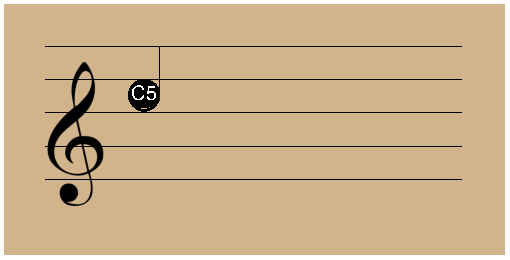
\includegraphics[trim=2.4000000000000004 2.4000000000000004 2.4000000000000004 2.4000000000000004]{pict.pdf}}}\end{SingleColumn}\end{RktBlk}\end{SCodeFlow}

Next, we place the notes in two different \RktSym{\badlink{\RktValLink{music}}}\RktMeta{} contexts with the two tunings we want to
try. \RktSym{\badlink{\RktValLink{namespace}}}\RktMeta{} is another type of context which is useful for certain things, though
just being used for show here.  \RktSym{\badlink{\RktValLink{name@}}}\RktMeta{} is a shorthand for ascribing a \RktSym{\badlink{\RktValLink{name}}}\RktMeta{} coordinate.

\begin{SCodeFlow}\begin{RktBlk}\begin{SingleColumn}\begin{RktBlk}\begin{SingleColumn}\RktPn{(}\RktSym{\badlink{\RktValLink{define{-}art}}}\mbox{\hphantom{\Scribtexttt{x}}}\RktSym{my{-}tunings}

\mbox{\hphantom{\Scribtexttt{xx}}}\RktPn{(}\RktSym{\badlink{\RktValLink{namespace}}}

\mbox{\hphantom{\Scribtexttt{xxxx}}}\RktPn{(}\RktSym{\badlink{\RktValLink{name@}}}\mbox{\hphantom{\Scribtexttt{x}}}\RktSym{12{-}tone{-}ET}

\mbox{\hphantom{\Scribtexttt{xxxxxx}}}\RktPn{(}\RktSym{\badlink{\RktValLink{music}}}\mbox{\hphantom{\Scribtexttt{x}}}\RktPn{(}\RktSym{\badlink{\RktValLink{tuning}}}\mbox{\hphantom{\Scribtexttt{x}}}\RktSym{12tet}\RktPn{)}\mbox{\hphantom{\Scribtexttt{x}}}\RktSym{my{-}notes}\RktPn{)}\RktPn{)}

\mbox{\hphantom{\Scribtexttt{xxxx}}}\RktPn{(}\RktSym{\badlink{\RktValLink{name@}}}\mbox{\hphantom{\Scribtexttt{x}}}\RktSym{Just{-}Intonation}

\mbox{\hphantom{\Scribtexttt{xxxxxx}}}\RktPn{(}\RktSym{\badlink{\RktValLink{music}}}\mbox{\hphantom{\Scribtexttt{x}}}\RktPn{(}\RktSym{\badlink{\RktValLink{tuning}}}\mbox{\hphantom{\Scribtexttt{x}}}\RktSym{5{-}limit}\RktPn{)}\mbox{\hphantom{\Scribtexttt{x}}}\RktSym{my{-}notes}\RktPn{)}\RktPn{)}\RktPn{)}\RktPn{)}\end{SingleColumn}\end{RktBlk}

\RktPn{(}\RktSym{scale}\mbox{\hphantom{\Scribtexttt{x}}}\RktVal{1/2}\mbox{\hphantom{\Scribtexttt{x}}}\RktPn{(}\RktSym{\badlink{\RktValLink{realize}}}\mbox{\hphantom{\Scribtexttt{x}}}\RktPn{(}\RktSym{\badlink{\RktValLink{draw{-}realizer}}}\mbox{\hphantom{\Scribtexttt{x}}}\RktPn{[}\RktVal{600}\mbox{\hphantom{\Scribtexttt{x}}}\RktVal{100}\RktPn{]}\RktPn{)}\mbox{\hphantom{\Scribtexttt{x}}}\RktSym{my{-}tunings}\RktPn{)}\RktPn{)}

\raisebox{-0.0bp}{\makebox[240.0bp][l]{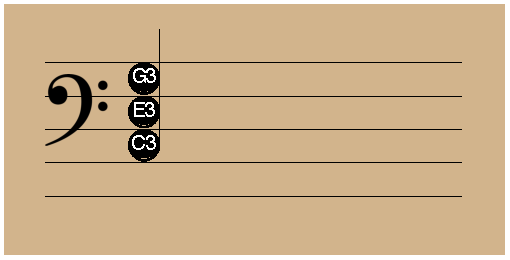
\includegraphics[trim=2.4000000000000004 2.4000000000000004 2.4000000000000004 2.4000000000000004]{pict_2.pdf}}}\end{SingleColumn}\end{RktBlk}\end{SCodeFlow}

Finally, we run \RktSym{\badlink{\RktValLink{note{-}{\Stttextmore}tone}}}\RktMeta{}.  Because of the way we wrote this art,
the code is slightly obfuscated with a few layers of \Scribtexttt{rewrite{-}in} destructuring.
\RktPn{(}\RktSym{\badlink{\RktValLink{delete}}}\RktMeta{}\mbox{\hphantom{\Scribtexttt{x}}}\RktMeta{}\RktSym{\badlink{\RktValLink{tuning}}}\RktPn{)}\RktMeta{} is done to declutter the resulting image.

\begin{SCodeFlow}\begin{RktBlk}\begin{SingleColumn}\begin{RktBlk}\begin{SingleColumn}\RktPn{(}\RktSym{scale}\mbox{\hphantom{\Scribtexttt{x}}}\RktVal{1/2}

\mbox{\hphantom{\Scribtexttt{xx}}}\RktPn{(}\RktSym{\badlink{\RktValLink{realize}}}\mbox{\hphantom{\Scribtexttt{x}}}\RktPn{(}\RktSym{\badlink{\RktValLink{draw{-}realizer}}}\mbox{\hphantom{\Scribtexttt{x}}}\RktPn{[}\RktVal{600}\mbox{\hphantom{\Scribtexttt{x}}}\RktVal{100}\RktPn{]}\RktPn{)}

\mbox{\hphantom{\Scribtexttt{xxxx}}}\RktSym{my{-}tunings}

\mbox{\hphantom{\Scribtexttt{xxxx}}}\RktPn{(}\RktSym{\badlink{\RktValLink{rewrite{-}in{-}namespace}}}

\mbox{\hphantom{\Scribtexttt{xxxxxx}}}\RktPn{(}\RktSym{\badlink{\RktValLink{rewrite{-}in{-}music}}}

\mbox{\hphantom{\Scribtexttt{xxxxxxxx}}}\RktPn{(}\RktSym{\badlink{\RktValLink{rewrite{-}in{-}seq}}}\mbox{\hphantom{\Scribtexttt{x}}}\RktPn{(}\RktSym{\badlink{\RktValLink{note{-}{\Stttextmore}tone}}}\RktPn{)}\RktPn{)}

\mbox{\hphantom{\Scribtexttt{xxxxxxxx}}}\RktPn{(}\RktSym{\badlink{\RktValLink{delete}}}\mbox{\hphantom{\Scribtexttt{x}}}\RktSym{\badlink{\RktValLink{tuning}}}\RktPn{)}\RktPn{)}\RktPn{)}\RktPn{)}\RktPn{)}\end{SingleColumn}\end{RktBlk}

\raisebox{-0.0bp}{\makebox[240.0bp][l]{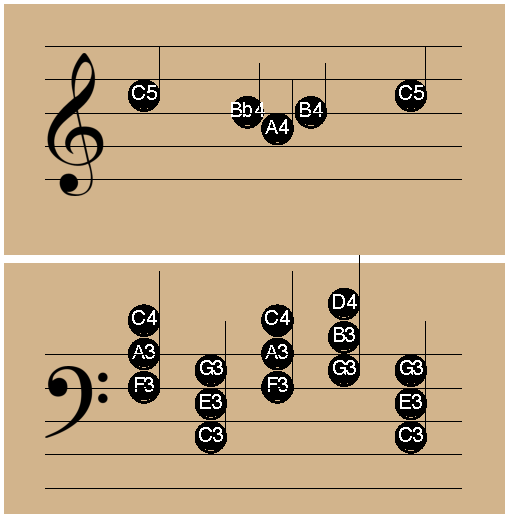
\includegraphics[trim=2.4000000000000004 2.4000000000000004 2.4000000000000004 2.4000000000000004]{pict_3.pdf}}}\end{SingleColumn}\end{RktBlk}\end{SCodeFlow}

One interesting thing to note is how the Just Intoned result is represented by
fractions, while the Equal Tempered result is represented by decimals.  This is
indirectly a result of the fact that Just Intonation is tuned with
multiplication by whole number ratios, while Equal Temperament is tuned using
multiplication by an irrational number.

\Ssubsubsection{Chords}{Chords}\label{t:x28part_x22Chordsx22x29}

Chords are an abstraction over combinations of notes, which often function like
a set of pitch classes.  For the purposes of this demo, our chord symbols will
specify sets of 3 pitch classes, called triads.

\begin{SCodeFlow}\begin{RktBlk}\begin{SingleColumn}\RktCmt{;;}\mbox{\hphantom{\Scribtexttt{x}}}\RktCmt{Standard}\mbox{\hphantom{\Scribtexttt{x}}}\RktCmt{Syntax}\RktMeta{}

\RktMeta{}\RktSym{{\Stttextless}pitch{-}label{\Stttextmore}{\Stttextless}accidental{\Stttextmore}{\Stttextless}quality{-}abbrev{\Stttextmore}}\RktMeta{}

\RktMeta{}\RktSym{or}\RktMeta{}

\RktMeta{}\RktSym{{\Stttextless}pitch{-}class{\Stttextmore}}\RktMeta{}\mbox{\hphantom{\Scribtexttt{x}}}\RktMeta{}\RktSym{{\Stttextless}quality{\Stttextmore}}\RktMeta{}

\RktMeta{}\RktCmt{;;}\mbox{\hphantom{\Scribtexttt{x}}}\RktCmt{Example}\RktMeta{}

\RktMeta{}\RktSym{F\#m}\RktMeta{}\mbox{\hphantom{\Scribtexttt{x}}}\RktMeta{}\RktSym{or}\RktMeta{}\mbox{\hphantom{\Scribtexttt{x}}}\RktMeta{}\RktSym{F\#}\RktMeta{}\mbox{\hphantom{\Scribtexttt{x}}}\RktMeta{}\RktSym{minor}\RktMeta{}

\RktMeta{~}

\RktMeta{}\RktCmt{;;}\mbox{\hphantom{\Scribtexttt{x}}}\RktCmt{Tonart}\mbox{\hphantom{\Scribtexttt{x}}}\RktCmt{Syntax}\RktMeta{}

\RktMeta{}\RktPn{(}\RktSym{\badlink{\RktValLink{chord}}}\RktMeta{}\mbox{\hphantom{\Scribtexttt{x}}}\RktMeta{}\RktSym{{\Stttextless}pitch{-}label{\Stttextmore}}\RktMeta{}\mbox{\hphantom{\Scribtexttt{x}}}\RktMeta{}\RktSym{{\Stttextless}accidental{-}number{\Stttextmore}}\RktMeta{}

\RktMeta{}\mbox{\hphantom{\Scribtexttt{xxxxxxx}}}\RktMeta{}\RktPn{[}\RktSym{{\Stttextless}quality{\Stttextmore}}\RktPn{]}\RktPn{)}\RktMeta{}

\RktMeta{}\RktCmt{;;}\mbox{\hphantom{\Scribtexttt{x}}}\RktCmt{Example}\RktMeta{}

\RktMeta{}\RktPn{(}\RktSym{\badlink{\RktValLink{chord}}}\RktMeta{}\mbox{\hphantom{\Scribtexttt{x}}}\RktMeta{}\RktSym{f}\RktMeta{}\mbox{\hphantom{\Scribtexttt{x}}}\RktMeta{}\RktVal{1}\RktMeta{}\mbox{\hphantom{\Scribtexttt{x}}}\RktMeta{}\RktPn{[}\RktSym{m}\RktPn{]}\RktPn{)}\RktMeta{}\end{SingleColumn}\end{RktBlk}\end{SCodeFlow}

Any number of notes can be in a chord, including repeats and octave
transpositions.  Each note must be a member of one of the pitch classes
corresponding to the chord.  Not all pitch classes from the set need be present
for a chord to retain its identity.  The pitch label of the chord is called
the "root" of the chord, and must be present.  The "quality" of the chord
deals with the intervals between notes in the chord.  C major, CM, or simply C,
has pitch classes C, E, and G.  C minor or Cm has pitch classes C, Eb, and G.
These are the two chord qualities that will be used in the demo.

Here is an example of chords being rewritten to notes.

\begin{SCodeFlow}\begin{RktBlk}\begin{SingleColumn}\begin{RktBlk}\begin{SingleColumn}\RktPn{(}\RktSym{\badlink{\RktValLink{define{-}art}}}\mbox{\hphantom{\Scribtexttt{x}}}\RktSym{my{-}chords}

\mbox{\hphantom{\Scribtexttt{xx}}}\RktPn{(}\RktSym{\badlink{\RktValLink{seq}}}\mbox{\hphantom{\Scribtexttt{x}}}\RktPn{(}\RktSym{\badlink{\RktValLink{chords}}}\mbox{\hphantom{\Scribtexttt{x}}}\RktPn{[}\RktSym{c}\mbox{\hphantom{\Scribtexttt{x}}}\RktVal{0}\mbox{\hphantom{\Scribtexttt{x}}}\RktSym{M}\RktPn{]}\mbox{\hphantom{\Scribtexttt{x}}}\RktPn{[}\RktSym{f}\mbox{\hphantom{\Scribtexttt{x}}}\RktVal{0}\mbox{\hphantom{\Scribtexttt{x}}}\RktSym{m}\RktPn{]}\mbox{\hphantom{\Scribtexttt{x}}}\RktPn{[}\RktSym{g}\mbox{\hphantom{\Scribtexttt{x}}}\RktVal{1}\mbox{\hphantom{\Scribtexttt{x}}}\RktSym{M}\RktPn{]}\RktPn{)}\RktPn{)}\RktPn{)}\end{SingleColumn}\end{RktBlk}

\RktPn{(}\RktSym{\badlink{\RktValLink{realize}}}\mbox{\hphantom{\Scribtexttt{x}}}\RktPn{(}\RktSym{\badlink{\RktValLink{draw{-}realizer}}}\mbox{\hphantom{\Scribtexttt{x}}}\RktPn{[}\RktVal{200}\mbox{\hphantom{\Scribtexttt{x}}}\RktVal{40}\RktPn{]}\RktPn{)}\mbox{\hphantom{\Scribtexttt{x}}}\RktSym{my{-}chords}\RktPn{)}

\raisebox{-0.7999999999999972bp}{\makebox[136.79999999999998bp][l]{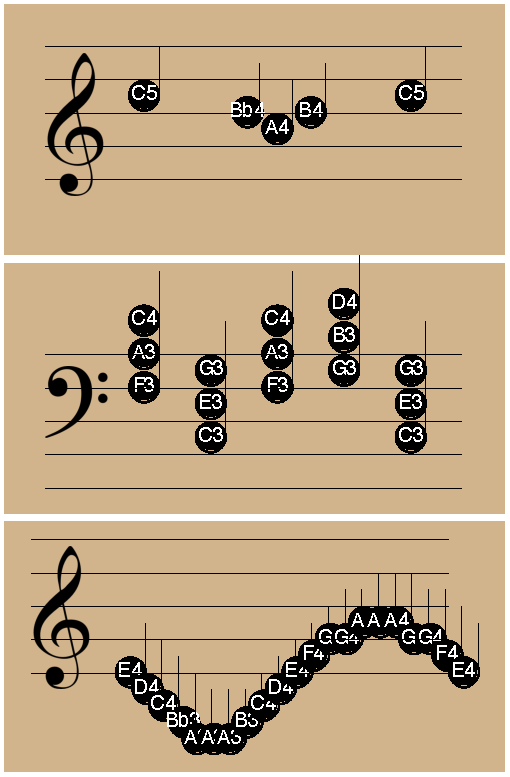
\includegraphics[trim=2.4000000000000004 2.4000000000000004 2.4000000000000004 2.4000000000000004]{pict_4.pdf}}}\end{SingleColumn}\end{RktBlk}\end{SCodeFlow}

Next we turn them into notes.  The particular choice of notes is, as mentioned,
arbitrary.  The \RktSym{\badlink{\RktValLink{chord{-}{\Stttextmore}notes/simple}}}\RktMeta{} rewriter happens to stack the first
three notes in the chord, ascenting from the given octave.

\begin{SCodeFlow}\begin{RktBlk}\begin{SingleColumn}\begin{RktBlk}\begin{SingleColumn}\RktPn{(}\RktSym{\badlink{\RktValLink{realize}}}\mbox{\hphantom{\Scribtexttt{x}}}\RktPn{(}\RktSym{\badlink{\RktValLink{draw{-}realizer}}}\mbox{\hphantom{\Scribtexttt{x}}}\RktPn{[}\RktVal{300}\mbox{\hphantom{\Scribtexttt{x}}}\RktVal{50}\RktPn{]}\RktPn{)}

\mbox{\hphantom{\Scribtexttt{xx}}}\RktPn{(}\RktSym{\badlink{\RktValLink{music}}}

\mbox{\hphantom{\Scribtexttt{xxxx}}}\RktSym{my{-}chords}

\mbox{\hphantom{\Scribtexttt{xxxx}}}\RktPn{(}\RktSym{\badlink{\RktValLink{rewrite{-}in{-}seq}}}\mbox{\hphantom{\Scribtexttt{x}}}\RktPn{(}\RktSym{\badlink{\RktValLink{chord{-}{\Stttextmore}notes/simple}}}\mbox{\hphantom{\Scribtexttt{x}}}\RktVal{4}\RktPn{)}\RktPn{)}\RktPn{)}\RktPn{)}\end{SingleColumn}\end{RktBlk}

\raisebox{-0.19999999999998863bp}{\makebox[240.0bp][l]{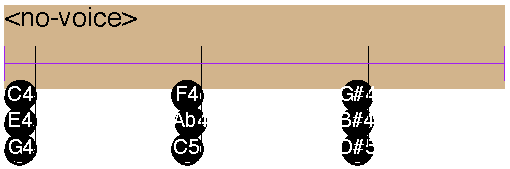
\includegraphics[trim=2.4000000000000004 2.4000000000000004 2.4000000000000004 2.4000000000000004]{pict_5.pdf}}}\end{SingleColumn}\end{RktBlk}\end{SCodeFlow}

\Ssubsubsection{Keys and Degrees}{Keys and Degrees}\label{t:x28part_x22Keysx5fandx5fDegreesx22x29}

A key in music is similar to a chord, being defined by a root pitch and a modality.

\begin{SCodeFlow}\begin{RktBlk}\begin{SingleColumn}\RktCmt{;;}\mbox{\hphantom{\Scribtexttt{x}}}\RktCmt{Standard}\mbox{\hphantom{\Scribtexttt{x}}}\RktCmt{Syntax}\RktMeta{}

\RktMeta{}\RktSym{{\Stttextless}pitch{-}class{\Stttextmore}}\RktMeta{}\mbox{\hphantom{\Scribtexttt{x}}}\RktMeta{}\RktSym{{\Stttextless}quality{\Stttextmore}}\RktMeta{}

\RktMeta{}\RktCmt{;;}\mbox{\hphantom{\Scribtexttt{x}}}\RktCmt{Example}\RktMeta{}

\RktMeta{}\RktSym{F\#}\RktMeta{}\mbox{\hphantom{\Scribtexttt{x}}}\RktMeta{}\RktSym{minor}\RktMeta{}

\RktMeta{~}

\RktMeta{}\RktCmt{;;}\mbox{\hphantom{\Scribtexttt{x}}}\RktCmt{Tonart}\mbox{\hphantom{\Scribtexttt{x}}}\RktCmt{Syntax}\RktMeta{}

\RktMeta{}\RktPn{(}\RktSym{\badlink{\RktValLink{key}}}\RktMeta{}\mbox{\hphantom{\Scribtexttt{x}}}\RktMeta{}\RktSym{{\Stttextless}pitch{-}label{\Stttextmore}}\RktMeta{}\mbox{\hphantom{\Scribtexttt{x}}}\RktMeta{}\RktSym{{\Stttextless}accidental{-}number{\Stttextmore}}\RktMeta{}\mbox{\hphantom{\Scribtexttt{x}}}\RktMeta{}\RktSym{{\Stttextless}quality{\Stttextmore}}\RktPn{)}\RktMeta{}

\RktMeta{}\RktCmt{;;}\mbox{\hphantom{\Scribtexttt{x}}}\RktCmt{Example}\RktMeta{}

\RktMeta{}\RktPn{(}\RktSym{\badlink{\RktValLink{key}}}\RktMeta{}\mbox{\hphantom{\Scribtexttt{x}}}\RktMeta{}\RktSym{f}\RktMeta{}\mbox{\hphantom{\Scribtexttt{x}}}\RktMeta{}\RktVal{1}\RktMeta{}\mbox{\hphantom{\Scribtexttt{x}}}\RktMeta{}\RktSym{m}\RktPn{)}\RktMeta{}\end{SingleColumn}\end{RktBlk}\end{SCodeFlow}

The difference between the two is a key contains a number of different chords.  Keys are a
broader description of a harmony, containing a large number of notes, intervals, chords, and
even idioms which interact

A degree or scale degree represents a pitch class, made relative to the root of a key.

\begin{SCodeFlow}\begin{RktBlk}\begin{SingleColumn}\RktSym{{\char'136}{\Stttextless}number{\Stttextmore}}\RktMeta{}\mbox{\hphantom{\Scribtexttt{x}}}\RktMeta{}\RktCmt{;}\mbox{\hphantom{\Scribtexttt{x}}}\RktCmt{Standard}\mbox{\hphantom{\Scribtexttt{x}}}\RktCmt{Syntax}\RktMeta{}

\RktMeta{}\RktSym{{\char'136}2}\RktMeta{}\mbox{\hphantom{\Scribtexttt{x}}}\RktMeta{}\RktCmt{;}\mbox{\hphantom{\Scribtexttt{x}}}\RktCmt{Example}\RktMeta{}

\RktMeta{~}

\RktMeta{}\RktPn{(}\RktSym{\badlink{\RktValLink{{\char'136}}}}\RktMeta{}\mbox{\hphantom{\Scribtexttt{x}}}\RktMeta{}\RktSym{{\Stttextless}number{\Stttextmore}}\RktPn{)}\RktMeta{}\mbox{\hphantom{\Scribtexttt{x}}}\RktMeta{}\RktCmt{;}\mbox{\hphantom{\Scribtexttt{x}}}\RktCmt{Tonart}\mbox{\hphantom{\Scribtexttt{x}}}\RktCmt{Syntax}\RktMeta{}

\RktMeta{}\RktPn{(}\RktSym{\badlink{\RktValLink{{\char'136}}}}\RktMeta{}\mbox{\hphantom{\Scribtexttt{x}}}\RktMeta{}\RktVal{2}\RktPn{)}\RktMeta{}\mbox{\hphantom{\Scribtexttt{x}}}\RktMeta{}\RktCmt{;}\mbox{\hphantom{\Scribtexttt{x}}}\RktCmt{Example}\RktMeta{}\end{SingleColumn}\end{RktBlk}\end{SCodeFlow}

We will show the first four degrees of three different keys: C major, B{-}flat
minor, and G{-}sharp major.

\begin{SCodeFlow}\begin{RktBlk}\begin{SingleColumn}\begin{RktBlk}\begin{SingleColumn}\RktPn{(}\RktSym{\badlink{\RktValLink{define{-}art}}}\mbox{\hphantom{\Scribtexttt{x}}}\RktSym{my{-}degrees}

\mbox{\hphantom{\Scribtexttt{xx}}}\RktPn{(}\RktSym{\badlink{\RktValLink{i@}}}\mbox{\hphantom{\Scribtexttt{x}}}\RktPn{[}\RktVal{0}\mbox{\hphantom{\Scribtexttt{x}}}\RktVal{12}\RktPn{]}

\mbox{\hphantom{\Scribtexttt{xxxx}}}\RktPn{(}\RktSym{\badlink{\RktValLink{voice@}}}\mbox{\hphantom{\Scribtexttt{x}}}\RktPn{(}\RktSym{alto}\RktPn{)}

\mbox{\hphantom{\Scribtexttt{xxxxxx}}}\RktPn{(}\RktSym{\badlink{\RktValLink{seq}}}\mbox{\hphantom{\Scribtexttt{x}}}\RktPn{(}\RktSym{\badlink{\RktValLink{{\char'136}s}}}\mbox{\hphantom{\Scribtexttt{x}}}\RktVal{1}\mbox{\hphantom{\Scribtexttt{x}}}\RktVal{2}\mbox{\hphantom{\Scribtexttt{x}}}\RktVal{3}\mbox{\hphantom{\Scribtexttt{x}}}\RktVal{4}\mbox{\hphantom{\Scribtexttt{x}}}\RktVal{1}\mbox{\hphantom{\Scribtexttt{x}}}\RktVal{2}\mbox{\hphantom{\Scribtexttt{x}}}\RktVal{3}\mbox{\hphantom{\Scribtexttt{x}}}\RktVal{4}\mbox{\hphantom{\Scribtexttt{x}}}\RktVal{1}\mbox{\hphantom{\Scribtexttt{x}}}\RktVal{2}\mbox{\hphantom{\Scribtexttt{x}}}\RktVal{3}\mbox{\hphantom{\Scribtexttt{x}}}\RktVal{4}\RktPn{)}\RktPn{)}

\mbox{\hphantom{\Scribtexttt{xxxxxx}}}\RktPn{(}\RktSym{\badlink{\RktValLink{urhy*}}}\mbox{\hphantom{\Scribtexttt{x}}}\RktVal{1}\RktPn{)}\mbox{\hphantom{\Scribtexttt{x}}}\RktPn{(}\RktSym{\badlink{\RktValLink{delete}}}\mbox{\hphantom{\Scribtexttt{x}}}\RktSym{\badlink{\RktValLink{seq}}}\RktPn{)}\RktPn{)}\RktPn{)}

\mbox{\hphantom{\Scribtexttt{xx}}}\RktPn{(}\RktSym{\badlink{\RktValLink{{-}{-}}}}\mbox{\hphantom{\Scribtexttt{x}}}\RktPn{[}\RktVal{4}\mbox{\hphantom{\Scribtexttt{x}}}\RktPn{(}\RktSym{\badlink{\RktValLink{key}}}\mbox{\hphantom{\Scribtexttt{x}}}\RktSym{c}\mbox{\hphantom{\Scribtexttt{x}}}\RktVal{0}\mbox{\hphantom{\Scribtexttt{x}}}\RktSym{M}\RktPn{)}\RktPn{]}\mbox{\hphantom{\Scribtexttt{x}}}\RktPn{[}\RktVal{4}\mbox{\hphantom{\Scribtexttt{x}}}\RktPn{(}\RktSym{\badlink{\RktValLink{key}}}\mbox{\hphantom{\Scribtexttt{x}}}\RktSym{b}\mbox{\hphantom{\Scribtexttt{x}}}\RktVal{\mbox{{-}1}}\mbox{\hphantom{\Scribtexttt{x}}}\RktSym{m}\RktPn{)}\RktPn{]}

\mbox{\hphantom{\Scribtexttt{xxxxxx}}}\RktPn{[}\RktVal{4}\mbox{\hphantom{\Scribtexttt{x}}}\RktPn{(}\RktSym{\badlink{\RktValLink{key}}}\mbox{\hphantom{\Scribtexttt{x}}}\RktSym{g}\mbox{\hphantom{\Scribtexttt{x}}}\RktVal{1}\mbox{\hphantom{\Scribtexttt{x}}}\RktSym{M}\RktPn{)}\RktPn{]}\RktPn{)}\RktPn{)}\end{SingleColumn}\end{RktBlk}

\begin{RktBlk}\begin{SingleColumn}\RktPn{(}\RktSym{scale}\mbox{\hphantom{\Scribtexttt{x}}}\RktVal{1/2}

\mbox{\hphantom{\Scribtexttt{xx}}}\RktPn{(}\RktSym{\badlink{\RktValLink{realize}}}\mbox{\hphantom{\Scribtexttt{x}}}\RktPn{(}\RktSym{\badlink{\RktValLink{draw{-}realizer}}}\mbox{\hphantom{\Scribtexttt{x}}}\RktPn{[}\RktVal{600}\mbox{\hphantom{\Scribtexttt{x}}}\RktVal{80}\RktPn{]}\RktPn{)}

\mbox{\hphantom{\Scribtexttt{xxxx}}}\RktPn{(}\RktSym{\badlink{\RktValLink{music}}}\mbox{\hphantom{\Scribtexttt{x}}}\RktSym{my{-}degrees}\RktPn{)}\RktPn{)}\RktPn{)}\end{SingleColumn}\end{RktBlk}

\raisebox{-0.0bp}{\makebox[240.0bp][l]{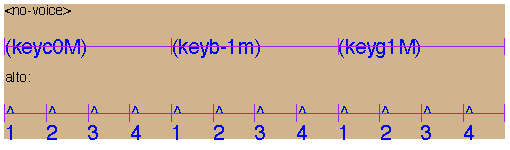
\includegraphics[trim=2.4000000000000004 2.4000000000000004 2.4000000000000004 2.4000000000000004]{pict_6.pdf}}}\end{SingleColumn}\end{RktBlk}\end{SCodeFlow}

\begin{SCodeFlow}\begin{RktBlk}\begin{SingleColumn}\begin{RktBlk}\begin{SingleColumn}\RktPn{(}\RktSym{scale}\mbox{\hphantom{\Scribtexttt{x}}}\RktVal{1/2}

\mbox{\hphantom{\Scribtexttt{xx}}}\RktPn{(}\RktSym{\badlink{\RktValLink{realize}}}\mbox{\hphantom{\Scribtexttt{x}}}\RktPn{(}\RktSym{\badlink{\RktValLink{draw{-}realizer}}}\mbox{\hphantom{\Scribtexttt{x}}}\RktPn{[}\RktVal{600}\mbox{\hphantom{\Scribtexttt{x}}}\RktVal{80}\RktPn{]}\RktPn{)}

\mbox{\hphantom{\Scribtexttt{xxxx}}}\RktPn{(}\RktSym{\badlink{\RktValLink{music}}}\mbox{\hphantom{\Scribtexttt{x}}}\RktSym{my{-}degrees}\mbox{\hphantom{\Scribtexttt{x}}}\RktPn{(}\RktSym{\badlink{\RktValLink{octave}}}\mbox{\hphantom{\Scribtexttt{x}}}\RktVal{4}\RktPn{)}

\mbox{\hphantom{\Scribtexttt{xxxxxxxxxxx}}}\RktPn{(}\RktSym{\badlink{\RktValLink{{\char'136}{-}{\Stttextmore}note}}}\RktPn{)}\mbox{\hphantom{\Scribtexttt{x}}}\RktPn{(}\RktSym{\badlink{\RktValLink{delete}}}\mbox{\hphantom{\Scribtexttt{x}}}\RktSym{\badlink{\RktValLink{octave}}}\RktPn{)}\RktPn{)}\RktPn{)}\RktPn{)}\end{SingleColumn}\end{RktBlk}

\raisebox{-0.20000000000000284bp}{\makebox[240.0bp][l]{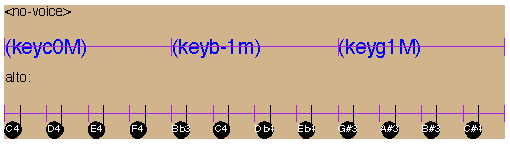
\includegraphics[trim=2.4000000000000004 2.4000000000000004 2.4000000000000004 2.4000000000000004]{pict_7.pdf}}}\end{SingleColumn}\end{RktBlk}\end{SCodeFlow}

\Ssubsubsection{Rhythm}{Rhythm}\label{t:x28part_x22Rhythmx22x29}

Rhythm is the timing and accentuation of specific beats.  The
Tonart rhythm object is a useful tool, but is very basic and only
captures the former.

\begin{SCodeFlow}\begin{RktBlk}\begin{SingleColumn}\RktPn{(}\RktSym{\badlink{\RktValLink{rhythm}}}\RktMeta{}\mbox{\hphantom{\Scribtexttt{x}}}\RktMeta{}\RktSym{{\Stttextless}number{\Stttextmore}}\RktMeta{}\mbox{\hphantom{\Scribtexttt{x}}}\RktMeta{}\RktSym{{\hbox{\texttt{.}}}{\hbox{\texttt{.}}}{\hbox{\texttt{.}}}}\RktPn{)}\RktMeta{}\mbox{\hphantom{\Scribtexttt{x}}}\RktMeta{}\RktCmt{;}\mbox{\hphantom{\Scribtexttt{x}}}\RktCmt{Tonart}\mbox{\hphantom{\Scribtexttt{x}}}\RktCmt{syntax}\RktMeta{}

\RktMeta{}\RktPn{(}\RktSym{\badlink{\RktValLink{rhythm}}}\RktMeta{}\mbox{\hphantom{\Scribtexttt{x}}}\RktMeta{}\RktVal{1}\RktMeta{}\mbox{\hphantom{\Scribtexttt{x}}}\RktMeta{}\RktVal{1}\RktMeta{}\mbox{\hphantom{\Scribtexttt{x}}}\RktMeta{}\RktVal{1/2}\RktMeta{}\mbox{\hphantom{\Scribtexttt{x}}}\RktMeta{}\RktVal{1/2}\RktMeta{}\mbox{\hphantom{\Scribtexttt{x}}}\RktMeta{}\RktVal{1}\RktMeta{}\mbox{\hphantom{\Scribtexttt{x}}}\RktMeta{}\RktVal{1}\RktPn{)}\RktMeta{}\mbox{\hphantom{\Scribtexttt{x}}}\RktMeta{}\RktCmt{;}\mbox{\hphantom{\Scribtexttt{x}}}\RktCmt{Example}\RktMeta{}\end{SingleColumn}\end{RktBlk}\end{SCodeFlow}

The series of numbers in the rhythm object denotes lengths
of time in beats.  A rewriter, \RktSym{\badlink{\RktValLink{apply{-}rhythm}}}\RktMeta{}, can be
used to place a sequence in time.

\begin{SCodeFlow}\begin{RktBlk}\begin{SingleColumn}\begin{RktBlk}\begin{SingleColumn}\RktPn{(}\RktSym{\badlink{\RktValLink{define{-}art}}}\mbox{\hphantom{\Scribtexttt{x}}}\RktSym{my{-}music}

\mbox{\hphantom{\Scribtexttt{xx}}}\RktPn{(}\RktSym{\badlink{\RktValLink{seq}}}\mbox{\hphantom{\Scribtexttt{x}}}\RktPn{(}\RktSym{\badlink{\RktValLink{notes}}}\mbox{\hphantom{\Scribtexttt{x}}}\RktPn{[}\RktSym{f}\mbox{\hphantom{\Scribtexttt{x}}}\RktVal{1}\mbox{\hphantom{\Scribtexttt{x}}}\RktVal{3}\RktPn{]}\mbox{\hphantom{\Scribtexttt{x}}}\RktPn{[}\RktSym{b}\mbox{\hphantom{\Scribtexttt{x}}}\RktVal{0}\mbox{\hphantom{\Scribtexttt{x}}}\RktVal{3}\RktPn{]}\mbox{\hphantom{\Scribtexttt{x}}}\RktPn{[}\RktSym{e}\mbox{\hphantom{\Scribtexttt{x}}}\RktVal{0}\mbox{\hphantom{\Scribtexttt{x}}}\RktVal{3}\RktPn{]}\mbox{\hphantom{\Scribtexttt{x}}}\RktPn{[}\RktSym{c}\mbox{\hphantom{\Scribtexttt{x}}}\RktVal{1}\mbox{\hphantom{\Scribtexttt{x}}}\RktVal{3}\RktPn{]}

\mbox{\hphantom{\Scribtexttt{xxxxxxxxxxxxxx}}}\RktPn{[}\RktSym{d}\mbox{\hphantom{\Scribtexttt{x}}}\RktVal{1}\mbox{\hphantom{\Scribtexttt{x}}}\RktVal{3}\RktPn{]}\mbox{\hphantom{\Scribtexttt{x}}}\RktPn{[}\RktSym{e}\mbox{\hphantom{\Scribtexttt{x}}}\RktVal{0}\mbox{\hphantom{\Scribtexttt{x}}}\RktVal{3}\RktPn{]}\mbox{\hphantom{\Scribtexttt{x}}}\RktPn{[}\RktSym{f}\mbox{\hphantom{\Scribtexttt{x}}}\RktVal{1}\mbox{\hphantom{\Scribtexttt{x}}}\RktVal{3}\RktPn{]}\RktPn{)}\RktPn{)}

\mbox{\hphantom{\Scribtexttt{xx}}}\RktPn{(}\RktSym{\badlink{\RktValLink{voice@}}}\mbox{\hphantom{\Scribtexttt{x}}}\RktPn{(}\RktSym{bass}\RktPn{)}

\mbox{\hphantom{\Scribtexttt{xxxx}}}\RktPn{(}\RktSym{\badlink{\RktValLink{rhythm}}}\mbox{\hphantom{\Scribtexttt{x}}}\RktVal{2}\mbox{\hphantom{\Scribtexttt{x}}}\RktVal{1/2}\mbox{\hphantom{\Scribtexttt{x}}}\RktVal{1/2}\mbox{\hphantom{\Scribtexttt{x}}}\RktVal{1}\mbox{\hphantom{\Scribtexttt{x}}}\RktVal{1/4}\mbox{\hphantom{\Scribtexttt{x}}}\RktVal{1/4}\mbox{\hphantom{\Scribtexttt{x}}}\RktVal{3}\RktPn{)}\RktPn{)}\RktPn{)}\end{SingleColumn}\end{RktBlk}

\begin{RktBlk}\begin{SingleColumn}\RktPn{(}\RktSym{scale}\mbox{\hphantom{\Scribtexttt{x}}}\RktVal{1/2}

\mbox{\hphantom{\Scribtexttt{xx}}}\RktPn{(}\RktSym{\badlink{\RktValLink{realize}}}\mbox{\hphantom{\Scribtexttt{x}}}\RktPn{(}\RktSym{\badlink{\RktValLink{draw{-}realizer}}}\mbox{\hphantom{\Scribtexttt{x}}}\RktPn{[}\RktVal{600}\mbox{\hphantom{\Scribtexttt{x}}}\RktVal{100}\RktPn{]}\RktPn{)}

\mbox{\hphantom{\Scribtexttt{xxxx}}}\RktPn{(}\RktSym{\badlink{\RktValLink{music}}}\mbox{\hphantom{\Scribtexttt{x}}}\RktSym{my{-}music}\RktPn{)}\RktPn{)}\RktPn{)}\end{SingleColumn}\end{RktBlk}

\raisebox{-0.19999999999998863bp}{\makebox[240.0bp][l]{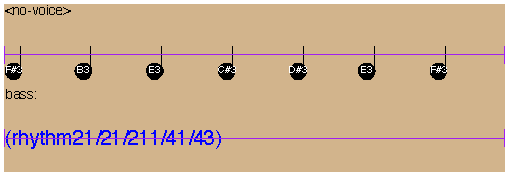
\includegraphics[trim=2.4000000000000004 2.4000000000000004 2.4000000000000004 2.4000000000000004]{pict_8.pdf}}}

\begin{RktBlk}\begin{SingleColumn}\RktPn{(}\RktSym{scale}\mbox{\hphantom{\Scribtexttt{x}}}\RktVal{1/2}

\mbox{\hphantom{\Scribtexttt{xx}}}\RktPn{(}\RktSym{\badlink{\RktValLink{realize}}}\mbox{\hphantom{\Scribtexttt{x}}}\RktPn{(}\RktSym{\badlink{\RktValLink{draw{-}realizer}}}\mbox{\hphantom{\Scribtexttt{x}}}\RktPn{[}\RktVal{600}\mbox{\hphantom{\Scribtexttt{x}}}\RktVal{100}\RktPn{]}\RktPn{)}

\mbox{\hphantom{\Scribtexttt{xxxx}}}\RktPn{(}\RktSym{\badlink{\RktValLink{music}}}\mbox{\hphantom{\Scribtexttt{x}}}\RktSym{my{-}music}\mbox{\hphantom{\Scribtexttt{x}}}\RktPn{(}\RktSym{\badlink{\RktValLink{apply{-}rhythm}}}\RktPn{)}\RktPn{)}\RktPn{)}\RktPn{)}\end{SingleColumn}\end{RktBlk}

\raisebox{-0.19999999999999574bp}{\makebox[240.0bp][l]{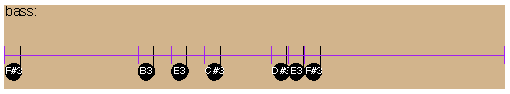
\includegraphics[trim=2.4000000000000004 2.4000000000000004 2.4000000000000004 2.4000000000000004]{pict_9.pdf}}}\end{SingleColumn}\end{RktBlk}\end{SCodeFlow}

\postDoc
\end{document}
